% !TeX program = pdflatex
% Parte VI de la serie godsil-gutman-lean. Versión en español, espejo fiel de
% gap-window-lean.tex.
% Las caminatas que recuerdan los ciclos — una ley del gap sharp verificada a máquina
% entre el polinomio de matchings y el espectro non-backtracking en Lean 4.
% Compilación: pdflatex gap-window-lean-es.tex (dos veces, por las referencias)

\documentclass[11pt]{article}
\usepackage[T1]{fontenc}
\usepackage[utf8]{inputenc}
\usepackage[spanish,es-noshorthands]{babel}
\usepackage{lmodern}
\usepackage{amsmath,amssymb,amsthm,booktabs,graphicx,hyperref}
\usepackage{xurl}
\usepackage[table]{xcolor}
\definecolor{ggteal}{HTML}{1B6F8C}
\definecolor{ggband}{HTML}{DCE7EB}
\definecolor{ggamber}{HTML}{E08A1E}
\usepackage[margin=1in]{geometry}
\usepackage{microtype}
\usepackage[most]{tcolorbox}
\usepackage{tikz}
\usetikzlibrary{arrows.meta,positioning}
\setlength{\emergencystretch}{2em}
\graphicspath{{figures/}}
\newtheorem{theorem}{Teorema}
\newtheorem{lemma}{Lema}
\newtheorem{definition}{Definición}
\newcommand{\lean}[1]{\texttt{#1}}
\newcommand{\Z}{\mathbb{Z}}
\newcommand{\R}{\mathbb{R}}
\newcommand{\N}{\mathbb{N}}
\newcommand{\C}{\mathbb{C}}
\DeclareMathOperator{\tr}{tr}
\hypersetup{colorlinks=true,linkcolor=ggteal,citecolor=ggteal,urlcolor=ggteal}
\newtcbox{\keybox}{on line,boxrule=0.9pt,colframe=ggteal,colback=ggband!40,
  arc=3pt,left=8pt,right=8pt,top=5pt,bottom=5pt}
\newcommand{\keyeq}[1]{\begin{center}\keybox{$\displaystyle #1$}\end{center}}

\title{\bf Las caminatas que recuerdan los ciclos\\[4pt]
  \large\normalfont Una ley del gap exacta verificada a máquina entre el polinomio
  de matchings\\ y el espectro non-backtracking en Lean~4}
\author{Carles Mar\'in\thanks{Formalizado con asistencia de IA (Claude, Anthropic); la
matemática y todas las afirmaciones son responsabilidad del autor. La metodología se discute
en la Sección~\ref{sec:boundary}.}\\[3pt]
  \normalsize Investigador independiente\\
  \normalsize \texttt{karlesmarin@gmail.com}}
\date{Junio de 2026}

\begin{document}
\maketitle

\begin{abstract}
Presento una demostración verificada a máquina, libre de \lean{sorry}, en Lean~4 sobre
Mathlib, de la \emph{ley del gap de fórmula de traza}, en su ventana exacta, para un grafo
simple finito de cuello (girth) $g$: para todo $1 \le k \le g+1$,
\[
\tr A^k \;-\; p_k \;=\; \tr B^k,
\]
donde $A$ es la matriz de adyacencia, $B$ el operador non-backtracking de Hashimoto y
$p_k = \sum_i \theta_i^k$ las sumas de potencias de las raíces del polinomio de matchings.
Por debajo del cuello ambos lados se anulan; en $k \in \{g, g+1\}$ ambos cuentan los
recorridos con punto base de los $k$-ciclos, $2k\,c_k$; y la ventana es exacta: la
ley falla en $k = g+2$ en todos los grafos comprobados, incluidos los $12\,064$ grafos
conexos con ciclos, de $4$ a $8$ vértices. La prueba se ensambla con piezas de uso
independiente: un lema de extracción de ciclos para cadenas non-backtracking; un lema de
paridad de incidencias para caminatas cerradas \emph{arbitrarias} (la versión de Mathlib
lleva una hipótesis de trail que su propia prueba no usa); un recuento exacto de incidencias
para ciclos; y un teorema de estructura: en la ventana, las caminatas cerradas
non-backtracking, los recorridos de ciclos con punto base y las caminatas cerradas que no
se elevan al árbol de caminos de Godsil son la \emph{misma} familia, contada de tres
maneras. El teorema principal depende solo de los tres axiomas estándar. Soy exacto con la
frontera: la matemática es clásica (Ihara, Hashimoto, Bass, Godsil; la ley es
folklore-adyacente y conocida por los teóricos de códigos con otra ropa); la contribución es
la formalización ---según mi mejor conocimiento, el primer puente verificado a máquina entre
el polinomio de matchings y el espectro non-backtracking en cualquier asistente de
pruebas--- y la ventana exacta se enuncia y demuestra como tal. Un artículo gemelo aplica la
ley, como censo certificado de ciclos cortos, a los códigos LDPC desplegados en el estándar
IEEE 802.11n (WiFi).
\end{abstract}

\noindent\emph{Mapa del lector.} Si solo va a leer una cosa, lea el
Teorema~\ref{thm:gaplaw} y la Figura~\ref{fig:window}: el enunciado, y la imagen de la ley
cumpliéndose en su ventana y rompiéndose, espectacularmente, justo después. La prueba es una
sola cadena (Figura~\ref{fig:readermap}); cada eslabón tiene su sección y su nombre Lean
(Tabla~\ref{tab:results}). Los límites honestos están en la Sección~\ref{sec:boundary}.

\begin{figure}[h]
\centering
\begin{tikzpicture}[
  theme/.style={draw=ggteal!70,fill=ggband!30,rounded corners=3pt,align=center,
    inner sep=5pt,font=\footnotesize,minimum height=9mm},
  hist/.style={draw=ggteal!70,fill=white,rounded corners=3pt,align=center,
    inner sep=5pt,font=\footnotesize,minimum height=9mm},
  last/.style={draw=ggamber,fill=ggamber!10,rounded corners=3pt,align=center,
    inner sep=5pt,font=\footnotesize,minimum height=9mm},
  flow/.style={-{Stealth[length=2.2mm]},semithick,ggteal!80}]
  \node[hist]  (a) at (0,1.5)    {1956--1992: una fórmula\\de traza baja a grafos\ \S\ref{sec:intro}};
  \node[theme] (b) at (4.05,1.5) {la afirmación:\\$\tr A^k - p_k = \tr B^k$\ \S\ref{sec:claim}};
  \node[theme] (c) at (8.1,1.5)  {bajo el cuello:\\ambos lados $=0$\ \S\ref{sec:stoneA}};
  \node[theme] (d) at (12.15,1.5){el muro: en la ventana\\toda caminata es ciclo\ \S\ref{sec:wall}};
  \node[theme] (e) at (12.15,-0.4){la elevación falla,\\el conteo cierra\ \S\ref{sec:count}};
  \node[theme] (f) at (8.1,-0.4) {asegurado: $12\,064$\\grafos + axiomas\ \S\ref{sec:verification}};
  \node[theme] (g) at (4.05,-0.4){dónde se aplica:\\WiFi, redes\ \S\ref{sec:applications}};
  \node[last]  (h) at (0,-0.4)   {límites y\\preguntas\ \S\ref{sec:boundary}--\ref{sec:questions}};
  \draw[flow] (a) -- (b);
  \draw[flow] (b) -- (c);
  \draw[flow] (c) -- (d);
  \draw[flow] (d) -- (e);
  \draw[flow] (e) -- (f);
  \draw[flow] (f) -- (g);
  \draw[flow] (g) -- (h);
\end{tikzpicture}
\caption{El mapa del lector: la afirmación, las tres piedras de su prueba, las
comprobaciones, los usos y lo que queda.}
\label{fig:readermap}
\end{figure}

% ---------------------------------------------------------------
\section{Introducción: una fórmula de traza baja por una escalera}
\label{sec:intro}

¿Por qué habrían de coincidir dos censos que no comparten ninguna definición? Empecemos por
la anomalía. Tómese el grafo de Petersen y háganse dos censos que no tienen ningún motivo
evidente para coincidir: cuéntense todas las caminatas cerradas de longitud
$k$ y réstense las que se elevan al árbol de caminos de Godsil ($\tr A^k - p_k$); por
separado, cuéntense las caminatas cerradas que nunca retroceden inmediatamente
($\tr B^k$). En $k = 5$ ambos dan $120$. En $k = 6$, ambos dan $120$ de nuevo. En $k = 7$
el primer censo salta a $1680$ ---y el segundo se desploma a $0$, porque el grafo de
Petersen no tiene ningún $7$-ciclo (Figura~\ref{fig:window}). Dos censos al unísono, y
luego un acantilado. El unísono es un teorema; el acantilado es su exactitud; este artículo
verifica ambos a máquina. ¿De dónde sale semejante par de censos?

En 1956 Selberg demostró una fórmula que enfrenta dos maneras de oír una superficie
hiperbólica: a un lado el espectro del laplaciano, al otro las longitudes de las geodésicas
cerradas~\cite{Selberg1956}. Diez años después Ihara, trabajando $p$-ádicamente, encontró la
sombra discreta de esa fórmula: una función zeta para un grafo, construida con sus
geodésicas cerradas, las caminatas cerradas que nunca retroceden
inmediatamente~\cite{Ihara1966}. Lo que era análisis sobre una superficie se volvió álgebra
lineal sobre un objeto finito: Hashimoto codificó la condición non-backtracking como una
matriz $0/1$ sobre las aristas dirigidas~\cite{Hashimoto1989}, y Bass demostró que su
polinomio característico factoriza a través de la matriz de adyacencia~\cite{Bass1992}: la
identidad de Selberg en versión grafo, formalizada en el companion Ihara--Bass de esta
serie~\cite{MarinBass2026}.

Una fórmula de traza necesita un segundo lado. En una superficie es el término de
Plancherel, la contribución del recubridor universal; en un grafo el recubridor universal es
un árbol, y el objeto que oye al árbol es el \emph{polinomio de matchings}: Godsil demostró
en 1981 que las sumas de potencias de sus raíces cuentan las caminatas cerradas que se
elevan al \emph{árbol de caminos}, las caminatas ``tree-like''~\cite{Godsil1981}, teorema
que esta serie formalizó en la Parte~IV~\cite{MarinMoment2026}, apoyándose en la biyección
del árbol de caminos de la Parte~III~\cite{MarinPTW2026} y en el carácter real de las raíces
de Heilmann y Lieb~\cite{HeilmannLieb1972}, formalizado en la Parte~II~\cite{MarinHL2026}.

Así que, llegada la Parte~V, la serie había construido por separado los dos lados de una
fórmula de traza: el lado árbol ($p_k$, polinomio de matchings, árbol de caminos) y el lado
geodésico ($\tr B^k$, operador non-backtracking, zeta de Ihara). Cada uno con su artículo,
sus verificaciones, su registro Zenodo. Nunca se habían encontrado dentro del asistente de
pruebas.

Este artículo es el encuentro. El puente es una resta:
\[
\tr A^k \;-\; p_k,
\]
todas las caminatas cerradas menos las tree-like: las caminatas que el árbol no puede
explicar. El teorema es que en una ventana exacta, $1 \le k \le g+1$ con $g$ el cuello, ese
resto \emph{es} la traza non-backtracking $\tr B^k$: lo que las caminatas olvidan del árbol
lo recuerdan de los ciclos. La ventana es exacta. Un paso más allá, en $k = g+2$, aparece la
primera caminata que envuelve un ciclo y luego deambula, y los dos lados se separan en todos
los grafos comprobados (Figura~\ref{fig:window}). La recompensa del collar es que este es el
primer teorema de la serie que \emph{consume las dos hebras a la vez}: su prueba Lean
importa la maquinaria de árbol de caminos y momentos de las Partes~III--IV y el operador de
Hashimoto del companion Ihara--Bass en el mismo archivo, y ninguno de los dos lados podría
enunciarse sin el vocabulario del otro.

% ---------------------------------------------------------------
\section{La afirmación: la ley y sus términos}
\label{sec:claim}

¿Qué se está restando, exactamente, en el lado izquierdo de la ley? En todo el artículo,
$G$ es un grafo simple finito con vértices $V$, $A$ su matriz de adyacencia y $g$ su cuello (la longitud de un ciclo más corto; $g \ge 3$). El polinomio de
matchings es
\[
\mu_G(x) \;=\; \sum_{j \ge 0} (-1)^j\, m_j\, x^{\,n-2j},
\]
con $m_j$ el número de matchings de $j$ aristas, y $p_k = \sum_{i} \theta_i^k$ la $k$-ésima
suma de potencias de sus raíces (sobre $\C$; de hecho las raíces son
reales~\cite{HeilmannLieb1972,MarinHL2026}). El operador de Hashimoto $B$ actúa sobre los
$2|E|$ \emph{dardos} (aristas ordenadas): $B_{d,e} = 1$ exactamente cuando $e$ continúa $d$
sin invertirlo ($\mathrm{snd}\,d = \mathrm{fst}\,e$ y
$e \neq \bar d$)~\cite{Hashimoto1989,MarinBass2026}.

\begin{theorem}[la ley del gap exacta; \lean{trace\_sub\_matchingPowerSum\_eq\_trace\_hashimoto}]
\label{thm:gaplaw}
Para todo $k$ con $1 \le k \le g+1$,
\keyeq{\tr A^k \;-\; p_k \;=\; \tr B^k .}
Por debajo del cuello ($k < g$) ambos lados son $0$. En $k \in \{g, g+1\}$ ambos lados valen
$2k\,c_k$, donde $c_k$ es el número de $k$-ciclos de $G$.
\end{theorem}

El enunciado Lean es exactamente este, sobre $\C$, con $p_k$ la \lean{Multiset.sum} literal
de las potencias $k$-ésimas de las raíces de \lean{matchingPoly} llevado a $\C$; la forma
entera \lean{treeLikeGap\_eq\_trace\_hashimoto} enuncia la misma identidad sobre $\Z$ con
$p_k$ sustituido por el conteo de caminatas tree-like de Godsil, y ambas se unen por el
teorema de momentos de la Parte~IV. No se asume regularidad, conexión ni bipartición. El
artefacto mismo, literal:
\begin{tcolorbox}[colframe=ggteal!70,colback=ggband!20,arc=3pt,boxrule=0.8pt]
\small\begin{verbatim}
theorem trace_sub_matchingPowerSum_eq_trace_hashimoto
    [Fintype V] [DecidableEq V] [DecidableRel G.Adj]
    {k : N} (hk : 0 < k) (hwin : (k : N_inf) <= G.egirth + 1) :
    ((G.adjMatrix N ^ k).trace : C) - G.matchingPowerSum k
      = ((G.hashimoto C) ^ k).trace
\end{verbatim}
\end{tcolorbox}

Un ejemplo cabe en la cabeza. En el triángulo $K_3$ con $k = g = 3$: hay seis caminatas
cerradas de longitud $3$ (tres puntos base, dos sentidos), así que $\tr A^3 = 6$; ninguna es
tree-like ---una vuelta al triángulo no se eleva a un árbol--- y en efecto $p_3 = 0$, pues
$\mu_{K_3} = x^3 - 3x$ tiene raíces $0, \pm\sqrt3$ cuyos cubos se cancelan; y las seis son
non-backtracking, así que $\tr B^3 = 6$. La ley dice $6 - 0 = 6$, y cada número se comprueba
sin papel. El teorema es que esto no falla nunca hasta $k = g+2$.

Tres observaciones antes de la prueba. Primera: la resta tiene sentido gracias a la
Parte~IV: $p_k$ \emph{es} un conteo de caminatas (las tree-like), de modo que el lado
izquierdo es la diferencia de dos censos de la misma población. Segunda: el lado derecho
también es un censo: $\tr B^k$ cuenta las caminatas cerradas non-backtracking de dardos de
longitud $k$ (\lean{trace\_hashimoto\_pow}, cartografiado en el companion
Jacobi--Newton~\cite{MarinJN2026}). El teorema es, por tanto, una \emph{biyección de
censos}, y así es como se demuestra. Tercera: la ventana importa: para $k \ge g+2$ la ley no
es que esté sin demostrar: es \emph{falsa}, y visiblemente
(Figura~\ref{fig:window}; Sección~\ref{sec:verification}); un único contraejemplo exacto
(Petersen en $k = 7$, donde $\tr A^7 - p_7 = 1680$ mientras $\tr B^7 = 0$) muestra que la
ventana no puede ensancharse. Que el fallo sea \emph{universal} más allá de $g+2$ está
comprobado en $12\,064$ grafos, no formalizado: el teorema es la igualdad en la ventana, y
``exacta'' (\emph{sharp}) significa que la ventana no puede extenderse.

\begin{figure}[t]
\centering
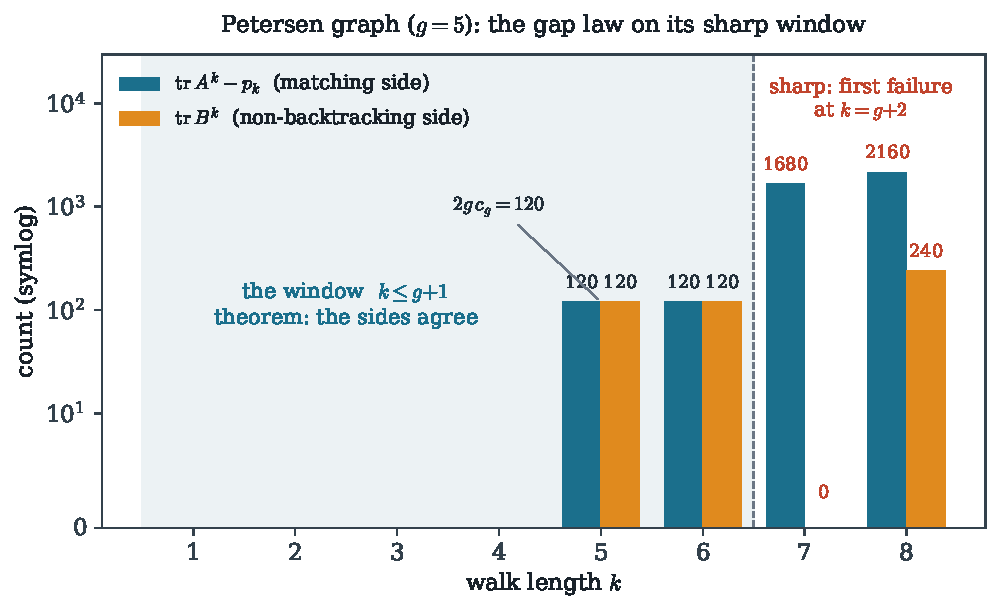
\includegraphics[width=0.92\textwidth]{gw_fig1_window}
\caption{La ley del gap en el grafo de Petersen ($g = 5$), en aritmética entera exacta. En
la ventana $k \le 6$ los dos censos coinciden: ambos son $0$ bajo el cuello y
$120 = 2\cdot 5\cdot 12$ en $k = 5$ (Petersen tiene doce pentágonos),
$120 = 2 \cdot 6 \cdot 10$ en $k = 6$ (diez hexágonos). En $k = 7$ la ley se rompe con toda
la violencia posible: el lado izquierdo salta a $1680$ mientras el derecho es $0$ ---el
grafo de Petersen, famosamente, no tiene $7$-ciclos, así que no existe ninguna caminata
cerrada non-backtracking de longitud $7$, mientras que $1680$ caminatas cerradas de longitud
$7$ ya no son tree-like (un pentágono más una arista colgante). La exactitud no es un
artefacto de un grafo: vale en los $12\,064$ grafos conexos con ciclos, de $4$ a $8$ vértices
(Sección~\ref{sec:verification}).}
\label{fig:window}
\end{figure}

\begin{table}[h]
\centering\small
\rowcolors{2}{ggband!35}{white}
\begin{tabular}{@{}rrrrr@{}}
\toprule
\rowcolor{ggteal!18} $k$ & $\tr A^k$ & $p_k$ & $\tr A^k - p_k$ & $\tr B^k$ \\
\midrule
1 & 0    & 0    & 0    & 0   \\
2 & 30   & 30   & 0    & 0   \\
3 & 0    & 0    & 0    & 0   \\
4 & 150  & 150  & 0    & 0   \\
5 & 120  & 0    & \textbf{120}  & \textbf{120} \\
6 & 990  & 870  & \textbf{120}  & \textbf{120} \\
7 & 1680 & 0    & {\color{ggamber}1680} & {\color{ggamber}0}   \\
8 & 7590 & 5430 & {\color{ggamber}2160} & {\color{ggamber}240} \\
\bottomrule
\end{tabular}
\caption{Los datos de Petersen tras la Figura~\ref{fig:window}: el espectro da
$\tr A^k = 3^k + 5 + 4(-2)^k$; $p_k$ por las identidades de Newton desde
$\mu = x^{10} - 15x^8 + 75x^6 - 145x^4 + 90x^2 - 6$; $\tr B^k$ por la recurrencia
por-autovalor de Ihara--Bass $s_k = \lambda s_{k-1} - 2 s_{k-2}$ más $5(1 + (-1)^k)$. La
ventana (negrita) y los dos primeros fallos (ámbar). Cada entrada es exacta.}
\label{tab:petersen}
\end{table}

% ---------------------------------------------------------------
\section{Piedra A: nada bajo el cuello}
\label{sec:stoneA}

Bajo el cuello la ley dice $0 = 0$; ¿por qué no es gratis ninguno de los dos ceros? Los
\emph{Árboles} de Serre enseñaron a una generación la consigna: por debajo de su cuello, un
grafo no puede distinguirse de su recubridor universal~\cite{Serre1980}. Una prueba formal
no puede señalar a un recubridor; necesita la consigna como testigo finito.

Tomemos primero el lado derecho: ¿por qué no existe ninguna caminata cerrada non-backtracking
más corta que el ciclo más corto? Clásicamente uno señala al recubridor universal; la prueba formal quiere un
testigo finito, y el testigo es un \emph{ciclo extraído de la propia caminata}.

\begin{lemma}[extracción de ciclos; \lean{Walk.exists\_isCycle\_of\_nbChain\_of\_not\_nodup}]
\label{lem:crux}
Sea $w$ una caminata cuyos dardos forman una cadena non-backtracking y cuyo soporte de
vértices repite un vértice. Entonces $G$ contiene un ciclo de longitud a lo sumo la de $w$,
soportado en las aristas de $w$.
\end{lemma}

La prueba es una inducción estructural sin ninguna rotación: rotar una caminata rompería la
cadena non-backtracking \emph{lineal} en la costura, una obstrucción que corrompe en
silencio las pruebas informales. Si la cola de la caminata ya repite un vértice, inducción.
Si no, el vértice de cabeza $u$ reentra en la cola; el prefijo hasta esa reentrada es un
camino (\lean{IsPath.takeUntil}), y la arista de cierre o bien evita el camino ---entonces
\lean{cons\_isCycle\_iff} nos entrega el ciclo--- o bien yace sobre él, lo que obliga al
camino a ser el único dardo invertido de la arista de entrada y contradice la cadena en su
primer eslabón. La Piedra~A se sigue por el principio del palomar: una caminata cerrada non-backtracking de
dardos de longitud $k$ presenta $k+1$ dardos cuyo último repite el primero, luego a lo sumo
$k$ aristas distintas; el ciclo extraído necesita al menos $g$ de ellas; así que $k \ge g$
(\lean{relWalks\_nbRel\_closed\_eq\_empty},
\lean{trace\_hashimoto\_pow\_eq\_zero\_of\_lt\_egirth}). El $0$ del lado izquierdo es el
teorema bajo-el-cuello de la Parte~III (toda caminata cerrada corta se eleva al árbol de
caminos). La ley del gap bajo el cuello es entonces una resta de ceros, pero cada cero es un
teorema.

% ---------------------------------------------------------------
\section{El muro: en la ventana, toda caminata es un ciclo}
\label{sec:wall}

¿Por qué una caminata cerrada non-backtracking de la ventana está obligada a ser un ciclo?
La cuchilla más vieja del libro es la de Euler, K\"onigsberg, 1736: toda entrada necesita
una salida~\cite{Euler1736}. Tres siglos después, el mismo argumento de paridad decide el
caso al que las hipótesis modernas no llegan.

El contenido de la ley vive en $k \in \{g, g+1\}$, y es un teorema de \emph{estructura}:

\begin{theorem}[rigidez de la ventana; \lean{Walk.isCycle\_of\_nbChain\_window}]
\label{thm:rigidity}
Una caminata cerrada non-backtracking de longitud $k$ con $1 \le k \le g+1$ es un ciclo.
\end{theorem}

Lo que nos sorprendió al formalizar es lo poco ``non-backtracking'' que usa la prueba al
final: la hipótesis de cadena entra \emph{solo} a través del Lema~\ref{lem:crux}. El ciclo
extraído $C$ cumple $g \le |C| \le k \le g+1$, lo que deja exactamente dos casos, y ambos
mueren contando incidencias de aristas: paridad y grado, nada más.

\emph{La cuchilla de paridad.} Para cualquier caminata, cuéntense las posiciones de arista
incidentes a un vértice $x$. Mathlib demuestra la paridad de este conteo para \emph{trails}
(\lean{IsTrail.even\_countP\_edges\_iff}), pero su propia inducción no usa la hipótesis de
trail más que para alimentarse a sí misma; al quitarla
(\lean{Walk.even\_countP\_edges\_iff'}) queda: en una caminata \emph{cerrada}, todo vértice
tiene conteo de incidencias par. Esto importa porque las caminatas del caso $|C| = k-1$ no
tienen por qué ser trails.

\emph{La cuchilla de grado.} Un ciclo toca cada vértice de su soporte en exactamente dos
posiciones de arista (\lean{Walk.countP\_edges\_of\_isCycle}), transferencia del
\lean{ncard\_neighborSet\_toSubgraph\_eq\_two} de Mathlib a lo largo de una biyección
explícita de dos lados, $e \mapsto$ ``el otro extremo''.

\emph{Caso $|C| = k-1$.} El multiconjunto de aristas de la caminata es el del ciclo más una
posición extra $f$ (una cirugía de multiconjuntos aísla $f$). Cualquier extremo $x$ de $f$
tiene entonces incidencia $2 + 1 = 3$ o $0 + 1 = 1$: impar en ambos casos, contra la
cuchilla de paridad. Tal caminata no existe
(\lean{Walk.not\_closed\_of\_isCycle\_edges\_add\_one}).

\emph{Caso $|C| = k$.} Las aristas de la caminata son una permutación de las del ciclo, así
que la caminata es un trail. Si su soporte repitiera un vértice interior $x$, rótese la
caminata a base $x$ (legítimo aquí: los trails sobreviven a la rotación, y ya no necesitamos
la cadena): $x$ queda en tres posiciones distintas dos a dos $\{0, m-1, m\}$, lo que da tres
aristas \emph{distintas} en $x$, contra las dos de la cuchilla de grado. Así que el soporte
es simple y la caminata es el ciclo (\lean{Walk.isCycle\_of\_edges\_perm}).

Componer los dos casos con el Lema~\ref{lem:crux} demuestra el Teorema~\ref{thm:rigidity}.
La hipótesis de ventana se usa exactamente una vez ---para encajar $|C|$ en
$\{k-1, k\}$--- y eso es precisamente lo que falla en $k = g+2$: se vuelve disponible un
$g$-ciclo más una excursión de $2$ pasos, la paridad queda satisfecha ($2+2$), y la ley se
rompe (Figuras~\ref{fig:window} y~\ref{fig:families}).

\begin{figure}[t]
\centering
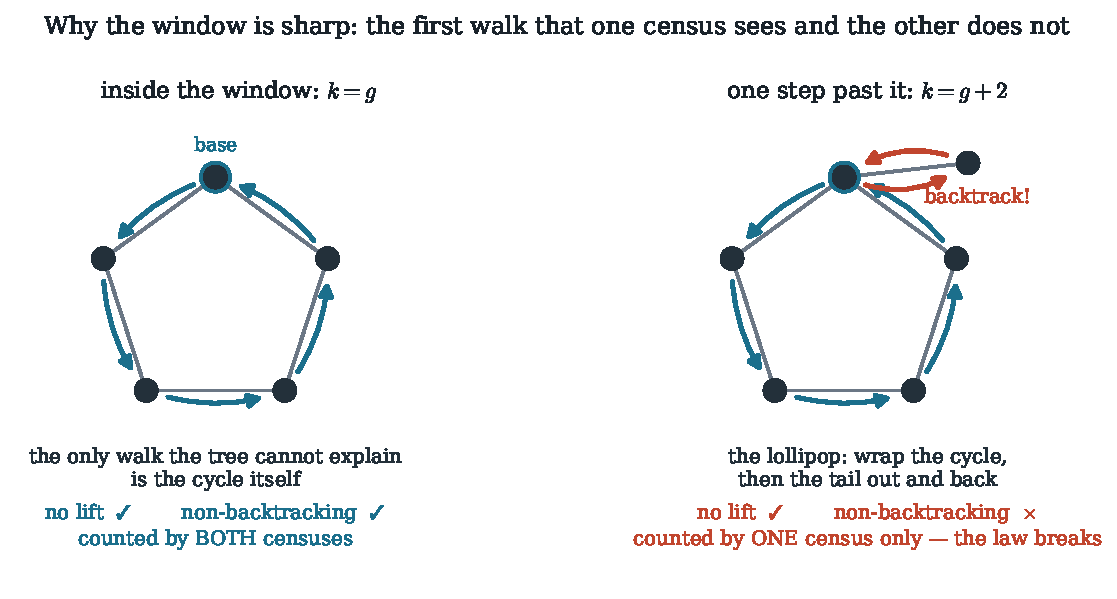
\includegraphics[width=0.92\textwidth]{gw_fig2_families}
\caption{El teorema de estructura en una imagen. Izquierda: dentro de la ventana, la única
caminata cerrada que el árbol de caminos no puede explicar es el recorrido de un ciclo, y un
ciclo nunca retrocede: los dos censos cuentan el mismo objeto. Derecha: en $k = g+2$ aparece
la primera \emph{piruleta}: envuelve el pentágono (no se eleva; el censo de matchings la
cuenta) pero su cola se da la vuelta sobre sí misma (el censo non-backtracking la rechaza).
Una caminata, un solo censo, ninguna ley.}
\label{fig:families}
\end{figure}

% ---------------------------------------------------------------
\section{El otro lado, y el conteo que cierra el puente}
\label{sec:count}

¿Cuándo se niega una caminata cerrada a elevarse al árbol de caminos, y por qué es eso
justamente lo que la hace un ciclo? Contar por biyección es el protocolo de confianza más
antiguo de la combinatoria: Pr\"ufer certificó el $n^{n-2}$ de Cayley exhibiendo la
correspondencia, árbol a árbol~\cite{Prufer1918}. La ley del gap cierra igual, caminata a caminata.

El censo izquierdo necesita el enunciado espejo: en la ventana, una caminata cerrada no se
eleva al árbol de caminos \emph{exactamente cuando} es un ciclo. Una dirección es un cálculo
agradable en la propia elevación: a lo largo de un ciclo la pila solo se extiende, y en el paso
de cierre la raíz está en la pila pero no es su penúltima entrada, así que la retirada falla
(\lean{Walk.not\_isTreeLike\_of\_isCycle}). La otra dirección necesitaba, sobre el papel, un
segundo muro, y se disolvió en piezas ya probadas: si una caminata de la ventana no se
eleva, su soporte de aristas contiene un ciclo (el contrapositivo del
\lean{isTreeLike\_of\_acyclic} de la Parte~III); llevar ese ciclo a $G$ aterriza exactamente
en los dos casos de la Sección~\ref{sec:wall}, cuyas conclusiones ahora se leen ``la
caminata es ese ciclo'' o ``falso''
(\lean{Walk.isCycle\_or\_isTreeLike\_window}).

Así que en la ventana coinciden tres familias:
\keyeq{\begin{aligned}
\{\text{caminatas NB cerradas de dardos}\} \;&=\; \{\text{recorridos de ciclos con punto base}\}\\
&=\; \{\text{caminatas cerradas que no se elevan}\},
\end{aligned}}
y la ley del gap es la afirmación de que la primera y la tercera tienen el mismo cardinal.
La biyección final (\lean{sum\_card\_not\_treeLike\_eq\_sum\_card\_relWalks}) envía una
caminata que no se eleva ---ya sabemos que es un ciclo--- a su lista de dardos cerrada con
la repetición de su primer dardo; la inyectividad descansa en un pequeño lema de valor
independiente, \emph{una caminata está determinada por sus dardos}
(\lean{Walk.eq\_of\_darts\_eq}); la sobreyectividad reensambla la caminata desde la lista de
dardos con el \lean{Walk.ofDarts} de Mathlib. Sumar sobre raíces y pasar por $\Z$ da el
teorema principal, y el teorema de momentos de la Parte~IV reescribe el conteo tree-like
como $p_k$: el Teorema~\ref{thm:gaplaw}.

\begin{table}[t]
\centering\small
\resizebox{\textwidth}{!}{%
\rowcolors{2}{ggband!35}{white}
\begin{tabular}{@{}lll@{}}
\toprule
\rowcolor{ggteal!18} nombre Lean & enunciado & dónde \\
\midrule
\lean{trace\_sub\_matchingPowerSum\_eq\_trace\_hashimoto} & $\tr A^k - p_k = \tr B^k$ en la ventana & \S\ref{sec:claim} \\
\lean{treeLikeGap\_eq\_trace\_hashimoto} & el teorema principal sobre $\Z$ & \S\ref{sec:claim} \\
\lean{exists\_isCycle\_of\_nbChain\_of\_not\_nodup} & extracción de ciclos de una cadena NB & \S\ref{sec:stoneA} \\
\lean{trace\_hashimoto\_pow\_eq\_zero\_of\_lt\_egirth} & $\tr B^k = 0$ para $k < g$ & \S\ref{sec:stoneA} \\
\lean{even\_countP\_edges\_iff'} & paridad de incidencias, sin hipótesis de trail & \S\ref{sec:wall} \\
\lean{countP\_edges\_of\_isCycle} & un ciclo tiene conteo de incidencias $2$ & \S\ref{sec:wall} \\
\lean{not\_closed\_of\_isCycle\_edges\_add\_one} & ninguna caminata es ciclo más una posición & \S\ref{sec:wall} \\
\lean{isCycle\_of\_edges\_perm} & caminata cerrada sobre las aristas de un ciclo $=$ el ciclo & \S\ref{sec:wall} \\
\lean{isCycle\_of\_nbChain\_window} & rigidez de la ventana (Teorema~\ref{thm:rigidity}) & \S\ref{sec:wall} \\
\lean{not\_isTreeLike\_of\_isCycle} & un ciclo no se eleva al árbol de caminos & \S\ref{sec:count} \\
\lean{isCycle\_or\_isTreeLike\_window} & la dicotomía de la ventana & \S\ref{sec:count} \\
\lean{eq\_of\_darts\_eq} & una caminata está determinada por sus dardos & \S\ref{sec:count} \\
\lean{sum\_card\_not\_treeLike\_eq\_sum\_card\_relWalks} & la biyección de censos & \S\ref{sec:count} \\
\bottomrule
\end{tabular}}
\caption{Los resultados que soportan carga, todos libres de \lean{sorry} en
\lean{Ihara/NbVanishing.lean} y \lean{Ihara/GapWindow.lean} del repositorio. Axiomas del
teorema principal: solo \lean{propext}, \lean{Classical.choice}, \lean{Quot.sound}.}
\label{tab:results}
\end{table}

% ---------------------------------------------------------------
\section{Asegurado: doce mil grafos y tres axiomas}
\label{sec:verification}

Si una prueba formal ya es cierta, ¿qué trabajo les queda a doce mil grafos? La evidencia
numérica es una brújula, no una escritura: la conjetura de Mertens estuvo de acuerdo con
todos los ordenadores que la miraron y cayó igualmente~\cite{OdlyzkoTeRiele1985}.
Los dos instrumentos se reparten aquí el trabajo en la dirección opuesta: la numérica elige
el enunciado; el asistente de pruebas lo posee.

Las pruebas formales eliminan una clase de error; elegir el \emph{enunciado correcto} exige
otro instrumento, y el enunciado de aquí ---en particular la afirmación de que la ventana es
exacta--- se fijó numéricamente antes de escribir una línea de Lean, y se re-verificó
después.

\begin{table}[h]
\centering\small
\rowcolors{2}{ggband!35}{white}
\begin{tabular}{@{}lrrrrr@{}}
\toprule
\rowcolor{ggteal!18} grafo & $g$ & $c_g$ & $\mathrm{gap}_g = \tr B^g$ & ventana verificada & primer fallo \\
\midrule
$K_3$        & 3 & 1  & 6   & $k \le 4$ & $k=5$ \\
$C_5$        & 5 & 1  & 10  & $k \le 6$ & $k=7$ \\
$K_4$        & 3 & 4  & 24  & $k \le 4$ & $k=5$ \\
$K_{3,3}$    & 4 & 9  & 72  & $k \le 5$ & $k=6$ \\
$Q_3$ (cubo) & 4 & 6  & 48  & $k \le 5$ & $k=6$ \\
Petersen     & 5 & 12 & 120 & $k \le 6$ & $k=7$ \\
\midrule
\multicolumn{6}{l}{\emph{barrido exhaustivo}: los $12\,064$ grafos conexos con ciclos, $4 \le n \le 8$
(Sage, \lean{nauty\_geng}):} \\
\multicolumn{6}{l}{\quad $0$ violaciones en la ventana; la ley falló en $k = g+2$ en
\emph{cada uno de los grafos}.} \\
\bottomrule
\end{tabular}
\caption{Las fijaciones numéricas. Los grafos con nombre se comprueban en aritmética exacta
(\lean{research/\_tmp/traceformula\_lock.py}); el barrido
(\lean{research/\_tmp/gaplaw\_sweep.py}) computa los dos lados de forma independiente
---$B$ como matriz explícita de dardos, $p_k$ por Newton desde los conteos de matchings--- y
confirma que la exactitud en $g+2$ es universal en este rango, no genérica.}
\label{tab:locks}
\end{table}

Por el lado formal: el desarrollo compila con Lean v4.30.0-rc2 contra un Mathlib fijado
(3054 trabajos, salida 0), los dos archivos nuevos están libres de avisos, y
\lean{\#print axioms} sobre cada teorema de la Tabla~\ref{tab:results} reporta
\lean{propext}, \lean{Classical.choice}, \lean{Quot.sound} ---los tres axiomas estándar--- y
nada más. Sin \lean{native\_decide}, sin bombas de decisión, sin axiomas propios.

Comprobar este artículo son tres órdenes:
\begin{tcolorbox}[colframe=ggteal!70,colback=ggband!20,arc=3pt,boxrule=0.8pt]
\footnotesize\begin{verbatim}
git clone https://github.com/karlesmarin/godsil-gutman-lean
cd godsil-gutman-lean && lake exe cache get && lake build Ihara
echo 'import Ihara.GapWindow
      #print axioms
        SimpleGraph.trace_sub_matchingPowerSum_eq_trace_hashimoto' \
  | lake env lean --stdin
\end{verbatim}
\end{tcolorbox}

% ---------------------------------------------------------------
\section{Dónde se aplica: de una identidad de trazas a un chip de WiFi}
\label{sec:applications}

¿Qué le da a un ingeniero una identidad de trazas verificada a máquina que un algoritmo más
rápido no? Gallager inventó los códigos LDPC en 1962 y el mundo los archivó treinta
años~\cite{Gallager1962}; cuando volvieron (al WiFi, al 5G, al espacio profundo), el cuello
de un grafo se había convertido en una cantidad de ingeniería. Ahí es donde una identidad de
trazas toca un chip.

\emph{Censos certificados de ciclos.} En $k = g$ la ley es una fórmula para el número de
ciclos más cortos, $c_g = (\tr A^g - p_g)/2g$, computable desde el espectro y los primeros
conteos de matchings. Los ciclos cortos en el grafo de Tanner de un código LDPC degradan la
decodificación por propagación de creencias, y contarlos es una tarea de ingeniería
establecida~\cite{KarimiBanihashemi2013,BlakeLin2018}. El artículo gemelo aplica la fórmula
(ahora respaldada por teorema) como \emph{censo certificado} a los cuatro códigos LDPC de
IEEE 802.11n con $n = 648$: tres cómputos mutuamente independientes coinciden exactamente en
los cuatro ---$c_6 = 3942$ (rate $1/2$), $c_6 = 8046$ (rate $2/3$), $c_4 = 54$ (rate $3/4$,
donde el cuello colapsa a $4$), $c_6 = 32\,346$ (rate $5/6$). La contribución allí es la
capa de certificación, no la velocidad: los algoritmos
de~\cite{KarimiBanihashemi2013,BlakeLin2018} son más rápidos y llegan más lejos
($k \le 2g-2$), pero no llevan garantía verificada a máquina.

\begin{tcolorbox}[colframe=ggamber,colback=ggamber!8,arc=3pt,boxrule=0.8pt,
  title=\textbf{La receta: cuente los ciclos más cortos de su grafo en cuatro líneas},
  coltitle=white,colbacktitle=ggamber]
Dado un grafo de cuello $g$ (caso par mostrado; $m_j$ = número de matchings de $j$ aristas):
(1) calcule $\tr A^g$ desde el espectro o por potencias de matrices;
(2) cuente los matchings pequeños, $m_1 = |E|$,
$m_2 = \binom{m_1}{2} - \sum_v \binom{d_v}{2}$, \dots\ hasta $m_{g/2}$;
(3) Newton: $p_2 = 2m_1$, $p_4 = 2m_1^2 - 4m_2$, $p_6 = 2m_1^3 - 6m_1m_2 + 6m_3$;
(4) entonces $c_g = (\tr A^g - p_g)/2g$, con garantía verificada a máquina.
\emph{Resuelto:} $K_{3,3}$ tiene $g = 4$, autovalores $\pm 3, 0^4$, así que
$\tr A^4 = 162$; $m_1 = 9$, $m_2 = \binom92 - 6\binom32 = 18$, luego
$p_4 = 2\cdot 81 - 4\cdot 18 = 90$; por tanto $c_4 = (162 - 90)/8 = 9$: los nueve
cuadriláteros de $K_{3,3}$, certificados.
\end{tcolorbox}

\emph{Química: el polinomio de matchings se mide.} En la teoría de H\"uckel de los
hidrocarburos conjugados, $\mu_G$ es el \emph{polinomio de referencia}: la energía de
resonancia topológica de una molécula es la diferencia entre los espectros de $A$ (el
sistema $\pi$) y de $\mu_G$ (el mismo sistema con los ciclos borrados): la aromaticidad como
distancia espectral entre un grafo y su propia sombra de árbol~\cite{Aihara1976,Gutman1979}.
La ley del gap es la identidad a nivel de caminatas bajo esa química: dice \emph{exactamente
qué} conteos de caminatas comparten los dos espectros (todos, hasta $g+1$) y dónde se
separan por primera vez. Los momentos $k$-ésimos del sistema $\pi$ del benceno y de su
polinomio de referencia coinciden hasta que $k = 6$ envuelve el hexágono: el sexteto
aromático, visto combinatoriamente.

\emph{Epidemias y percolación.} El umbral de percolación de una red dispersa y el umbral
epidémico de un proceso SIR están gobernados ambos por $1/\lambda_1(B)$, el autovalor
principal del operador non-backtracking~\cite{KarrerNewman2014}. Las estimaciones numéricas
de $\lambda_1(B)$ en una red grande son exactamente la situación donde importan los momentos
bajos certificados: $\tr B^g = 2g\,c_g$ y $\tr B^{g+1}$ fijan los primeros momentos no
triviales de la distribución espectral desde cantidades ($\tr A^k$, matchings pequeños)
calculadas por rutas de código independientes y bien probadas.

\emph{Métodos non-backtracking en ciencia de redes.} El operador $B$ se ha vuelto
herramienta estándar: las caminatas aleatorias non-backtracking mezclan más
rápido~\cite{ABLS2007}, y el espectro de $B$ alcanza el umbral de detectabilidad en
detección de comunidades donde los métodos de adyacencia fallan~\cite{Krzakala2013}. La ley
del gap da los momentos más pequeños de $B$ exactos, en términos de cantidades clásicas y
bien entendidas ($\tr A^k$ y matchings): las comprobaciones de cordura de nivel de entrada
para cualquier implementación numérica de $B$.

\emph{La conexión Ramanujan.} La Parte~I de esta serie formalizó la banda
$2\sqrt{d-1}$~\cite{MarinGG2026}; los grafos que la alcanzan (grafos de Ramanujan, con las
construcciones explícitas de Lubotzky--Phillips--Sarnak alcanzando cuello
$\sim \tfrac43 \log_{d-1} n$~\cite{LPS1988}) tienen cuello casi óptimo y, por tanto, las
\emph{ventanas certificadas más anchas} para esta ley.
El diseño garantiza pocos ciclos cortos; la ley del gap cuenta exactamente cuántos. Las dos
alas ---cota espectral e identidad de trazas--- están ahora verificadas a máquina, en el
mismo repositorio.

% ---------------------------------------------------------------
\section{La frontera honesta}
\label{sec:boundary}

Si la matemática es clásica, ¿dónde vive exactamente la contribución nueva?

\emph{La matemática es clásica.} La lectura como fórmula de traza del polinomio de matchings
frente a la zeta de Ihara está implícita en la literatura en torno a
Godsil~\cite{Godsil1981,GodsilBook}, Bass~\cite{Bass1992},
Stark--Terras~\cite{StarkTerras1996} y el libro de Terras~\cite{Terras2011}; los teóricos de
códigos conocen el censo $k \le g+1$ con otra ropa~\cite{BlakeLin2018}. No reclamo
matemática nueva. La contribución es el puente verificado a máquina, y la disciplina que la
formalización impuso (la obstrucción de la costura a la rotación, el lema de paridad sin
trail, el punto exacto donde entra la hipótesis de ventana), que es donde vive la novedad
genuina de este tipo de trabajo.

\emph{La ventana es $k \le g+1$, punto.} Los ingenieros cuentan hasta $2g-2$ con términos de
corrección~\cite{BlakeLin2018,Dehghan2018}; nada de eso está formalizado aquí, y la ley tal
como se enuncia es \emph{falsa} más allá de la ventana.

\emph{Formalizaciones previas.} No pude localizar ningún enunciado verificado a máquina que
conecte el polinomio de matchings con el operador non-backtracking, en ningún asistente de
pruebas. La afirmación de prioridad descansa menos en una búsqueda negativa que en un hecho
estructural: el operador non-backtracking $B$ no está, que yo sepa, formalizado en ningún
asistente ($B$ entra en Lean solo en el companion Ihara--Bass de esta serie), de modo que un
puente que lo consuma no puede ser anterior. Las búsquedas del 2026-06-11/12 sobre Mathlib, los
repositorios de la comunidad Lean, el AFP de Isabelle, Coq y HOL~Light no encontraron ni la
ley ni sus ingredientes. Tal afirmación solo puede hacerse según el mejor conocimiento de
uno.

\emph{Metodología.} La formalización se llevó a cabo con asistencia de IA (Claude,
Anthropic) bajo la disciplina usada en toda la serie: cada enunciado fijado por numérica
exacta antes de formalizar; cada teorema comprobado con \lean{\#print axioms}; cada
``primero'' reclamado, contrastado con la literatura antes de reclamarlo. La matemática y
todos los errores son míos.

% ---------------------------------------------------------------
\section{Preguntas abiertas}
\label{sec:questions}

\begin{enumerate}
\item \emph{La ventana corregida.} Para $g+2 \le k \le 2g-2$ el fallo tiene estructura: el
defecto $\tr A^k - p_k - \tr B^k$ cuenta caminatas piruleta, y se conocen correcciones en
forma cerrada de manera informal~\cite{BlakeLin2018,Dehghan2018}. Formalícese el primer
término de corrección. ¿Qué familia de caminatas cuenta exactamente el defecto de
$k = g+2$, en el vocabulario de Lean?
\item \emph{De trazas a geodésicas.} $\tr B^k$ cuenta caminatas non-backtracking \emph{con
punto base}; la zeta de Ihara quiere sus clases de rotación (geodésicas primas), a una
inversión de M\"obius de distancia. La maquinaria de órbitas cíclicas está a medio construir
en este repositorio (\lean{MathlibPR/MatrixWalkCount.lean}); el paso de Burnside ponderado
está abierto. ¿Puede el propio producto de Euler hacerse teorema?
\item \emph{Subir a Mathlib.} \lean{eq\_of\_darts\_eq}, el lema de paridad sin trail, el
conteo de incidencias de ciclos y la pequeña biblioteca de conteo de caminatas dirigidas
tienen forma de Mathlib. ¿Cuáles sobreviven a la revisión, y con qué generalidad?
\item \emph{La ventana como invariante.} El par $(\tr B^g, \tr B^{g+1}) = (2g\,c_g,\,
2(g{+}1)c_{g+1})$ es un invariante de grafos barato y certificado. ¿Cuánto de la clase de
isomorfismo de los grafos pequeños fija la ventana certificada, y dónde deja de distinguir
por primera vez?
\item \emph{Una para guardar.} Una resta es una medición: la ley del gap dice que un grafo
puede contar sus propios ciclos más cortos olvidando sus árboles. El lado árbol ($p_k$) es
el recubridor universal hablando; el lado ciclo ($\tr B^k$) es el grupo fundamental
respondiendo. ¿En qué $k$ ---en general, no solo pasado $g+1$--- deja un grafo finito de ser
explicable por su propio recubridor universal?
\item \emph{Lo que la formalización vio y el papel no.} Tres veces en esta prueba la
disciplina formal forzó un enunciado más afilado que el informal: la obstrucción del
\emph{seam} que prohíbe rotar una cadena non-backtracking, la hipótesis de \emph{trail} que
el lema de paridad de Mathlib arrastra pero nunca usa, y el punto único donde entra la
hipótesis de ventana. ¿Qué otros argumentos clásicos de este círculo de ideas de zetas de
grafos esconden una hipótesis no usada o una rotación silenciosa que solo un asistente de
pruebas detectaría?
\end{enumerate}

\section*{Disponibilidad de datos y código}
Las fuentes Lean (\lean{Ihara/NbVanishing.lean}, \lean{Ihara/GapWindow.lean}, con los
archivos de las Partes~III--V y el companion Ihara--Bass que importan), las fijaciones
numéricas y los scripts de las
figuras están en el repositorio público
\url{https://github.com/karlesmarin/godsil-gutman-lean}. El artículo gemelo aplicado (el
censo LDPC certificado) se referencia allí.

\begin{thebibliography}{99}\small

\bibitem{Euler1736} L. Euler,
\emph{Solutio problematis ad geometriam situs pertinentis},
Comment. Acad. Sci. Petrop. \textbf{8} (1736) 128--140.

\bibitem{Prufer1918} H. Pr\"ufer,
\emph{Neuer Beweis eines Satzes \"uber Permutationen},
Arch. Math. Phys. \textbf{27} (1918) 742--744.

\bibitem{Gallager1962} R.~G. Gallager,
\emph{Low-density parity-check codes}, IRE Trans. Inform. Theory \textbf{8} (1962) 21--28.

\bibitem{Serre1980} J.-P. Serre,
\emph{Trees}, Springer, 1980 (original francés \emph{Arbres, amalgames, $SL_2$}, 1977).

\bibitem{OdlyzkoTeRiele1985} A.~M. Odlyzko, H.~J.~J. te Riele,
\emph{Disproof of the Mertens conjecture}, J. Reine Angew. Math. \textbf{357} (1985)
138--160.

\bibitem{Aihara1976} J. Aihara,
\emph{A new definition of Dewar-type resonance energies},
J. Amer. Chem. Soc. \textbf{98} (1976) 2750--2758.

\bibitem{Gutman1979} I. Gutman,
\emph{The matching polynomial}, MATCH Commun. Math. Comput. Chem. \textbf{6} (1979)
75--91.

\bibitem{LPS1988} A. Lubotzky, R. Phillips, P. Sarnak,
\emph{Ramanujan graphs}, Combinatorica \textbf{8} (1988) 261--277.

\bibitem{KarrerNewman2014} B. Karrer, M.~E.~J. Newman, L. Zdeborov\'a,
\emph{Percolation on sparse networks}, Phys. Rev. Lett. \textbf{113} (2014) 208702.

\bibitem{Selberg1956} A. Selberg,
\emph{Harmonic analysis and discontinuous groups in weakly symmetric Riemannian spaces with
applications to Dirichlet series}, J. Indian Math. Soc. \textbf{20} (1956) 47--87.

\bibitem{Ihara1966} Y. Ihara,
\emph{On discrete subgroups of the two by two projective linear group over $p$-adic fields},
J. Math. Soc. Japan \textbf{18} (1966) 219--235.

\bibitem{HeilmannLieb1972} O.~J. Heilmann, E.~H. Lieb,
\emph{Theory of monomer-dimer systems}, Comm. Math. Phys. \textbf{25} (1972) 190--232.

\bibitem{Godsil1981} C.~D. Godsil,
\emph{Matchings and walks in graphs}, J. Graph Theory \textbf{5} (1981) 285--297.

\bibitem{GodsilBook} C.~D. Godsil,
\emph{Algebraic Combinatorics}, Chapman \& Hall, 1993.

\bibitem{Hashimoto1989} K. Hashimoto,
\emph{Zeta functions of finite graphs and representations of $p$-adic groups},
Adv. Stud. Pure Math. \textbf{15} (1989) 211--280.

\bibitem{Bass1992} H. Bass,
\emph{The Ihara--Selberg zeta function of a tree lattice},
Internat. J. Math. \textbf{3} (1992) 717--797.

\bibitem{StarkTerras1996} H.~M. Stark, A. Terras,
\emph{Zeta functions of finite graphs and coverings}, Adv. Math. \textbf{121} (1996)
124--165.

\bibitem{KotaniSunada2000} M. Kotani, T. Sunada,
\emph{Zeta functions of finite graphs}, J. Math. Sci. Univ. Tokyo \textbf{7} (2000) 7--25.

\bibitem{Terras2011} A. Terras,
\emph{Zeta Functions of Graphs: A Stroll through the Garden}, Cambridge Univ. Press, 2011.

\bibitem{ABLS2007} N. Alon, I. Benjamini, E. Lubetzky, S. Sodin,
\emph{Non-backtracking random walks mix faster}, Commun. Contemp. Math. \textbf{9} (2007)
585--603.

\bibitem{Krzakala2013} F. Krzakala, C. Moore, E. Mossel, J. Neeman, A. Sly, L. Zdeborov\'a,
P. Zhang, \emph{Spectral redemption in clustering sparse networks},
Proc. Natl. Acad. Sci. \textbf{110} (2013) 20935--20940.

\bibitem{KarimiBanihashemi2013} M. Karimi, A.~H. Banihashemi,
\emph{Message-passing algorithms for counting short cycles in a graph},
IEEE Trans. Commun. \textbf{61} (2013) 485--495.

\bibitem{BlakeLin2018} I.~F. Blake, S. Lin,
\emph{On short cycle enumeration in biregular bipartite graphs},
IEEE Trans. Inform. Theory \textbf{64} (2018) 6526--6535.

\bibitem{Dehghan2018} A. Dehghan, A.~H. Banihashemi,
\emph{On computing the multiplicity of cycles in bipartite graphs using the degree
distribution and the spectrum of the graph}, IEEE Trans. Inform. Theory \textbf{65} (2019)
3778--3789.

\bibitem{Mathlib2020} The mathlib community,
\emph{The Lean mathematical library}, en: CPP 2020, ACM, 2020, 367--381.

\bibitem{Lean4} L. de Moura, S. Ullrich,
\emph{The Lean 4 theorem prover and programming language}, en: CADE-28, LNCS 12699,
Springer, 2021, 625--635.

\bibitem{MarinGG2026} C. Mar\'in,
\emph{Random signs into matchings: a Godsil--Gutman identity, formalized in Lean~4}
(Parte I de esta serie), Zenodo, 2026. \texttt{doi:10.5281/zenodo.20517350}.

\bibitem{MarinHL2026} C. Mar\'in,
\emph{Unfolding a graph into a tree: a machine-checked proof of the Heilmann--Lieb theorem
in Lean~4} (Parte II), Zenodo, 2026. \texttt{doi:10.5281/zenodo.20561832}.

\bibitem{MarinPTW2026} C. Mar\'in,
\emph{Walks that forget the cycles: a machine-checked bijection between tree-like walks and
Godsil's path tree in Lean~4} (Parte III), Zenodo, 2026. \texttt{doi:10.5281/zenodo.20600326}.

\bibitem{MarinBass2026} C. Mar\'in,
\emph{Folding edges into vertices: a machine-checked proof of Bass's determinant formula
for the Ihara zeta function in Lean~4} (el companion Ihara--Bass de esta serie), Zenodo,
2026. \texttt{doi:10.5281/zenodo.20573120}.

\bibitem{MarinJN2026} C. Mar\'in,
\emph{What a determinant's derivative knows: Jacobi's formula and Newton's identity for
matrix traces in Lean 4}, Zenodo, 2026. \texttt{doi:10.5281/zenodo.20578470}.

\bibitem{MarinMoment2026} C. Mar\'in,
\emph{When walks become a spectrum: a machine-checked proof of Godsil's moment theorem in
Lean~4} (Parte IV), Zenodo, 2026. \texttt{doi:10.5281/zenodo.20613246}.

\bibitem{MarinMT2026} C. Mar\'in,
\emph{Counting trees without listing them: a machine-checked proof of Kirchhoff's
matrix-tree theorem in Lean~4} (Parte V), Zenodo, 2026. \texttt{doi:10.5281/zenodo.20629746}.

\end{thebibliography}

\end{document}
